\section{Model Exercise 1-2 (06): The drying and wetting paths of Opalinus Claystone}
\label{sec:mex06}
%------------------------------------------------------------------------------
\Authors{Amir Sattari et al.}
%------------------------------------------------------------------------------

The drying and wetting process and developed micro pathways in Opalinus claystone are the focus of the this model exercise (MEX 1-2). The simulation of the fracking during the shrinkage and swelling processes using the experimental data is carried out. Additionally, the change of hydraulic conductivity both in parallel and perpendicular to the embedded layering orientations is investigated. It is shown that due to the inherent anisotropy of claystone material, the materials behavior in parallel and perpendicular orientations are different.  

%------------------------------------------------------------------------------
\subsection{Experimental set-up}
%------------------------------------------------------------------------------
The prepared two cylindrical thin sections of sandy Opalinus claystone (see Figure \ref{fig:Amir_Shrinkage_Full_Setup}) are used to determine the drying and wetting paths. The saturated salt solutions are used to apply different osmotic suctions (see Table \ref{table:Amir_Shrinkage_SaltSolutions}). The suction values range from 3.2 up to 367 $MPa$, which insures both drying and wetting paths. The room temperature is around 20 $^{\circ}C$ and the fluctuation of the temperature is negligible. The first sample is used to determine the linear axial strains (see \ref{fig:Amir_Shrinkage_Sensors}) along the embedded layers, which are arranged in a parallel and perpendicular orientations. The second sample is used to determine the water content change during the wetting and drying paths. The samples dimension is 100x10 $mm$ $(DxH)$. The equilibrium inside the desiccator is reached when the change of the samples water content is zero. Figure \ref{fig:Amir_ME6_Strain} depicts the change of suction and axial linear strains in parallel and perpendicular directions. Similarly, Figure \ref{fig:Amir_ME6_Water} shows the change of water content with applied suction using salt solutions. In drying path, the results indicate a higher strains for a strain perpendicular to the embedded layers. When the suction is higher than 150 $MPa$, the strains in perpendicular direction are almost 4.5 larger than parallel ones. Interestingly, in the wetting path, the differences between the strain gauges are much less.  According to the water content data, the air-entry pressure for a sandy Opalinus claystone is around 25 $MPa$.

\begin{figure}[!ht]
\begin{subfigure}[c]{0.48\textwidth}
\centering
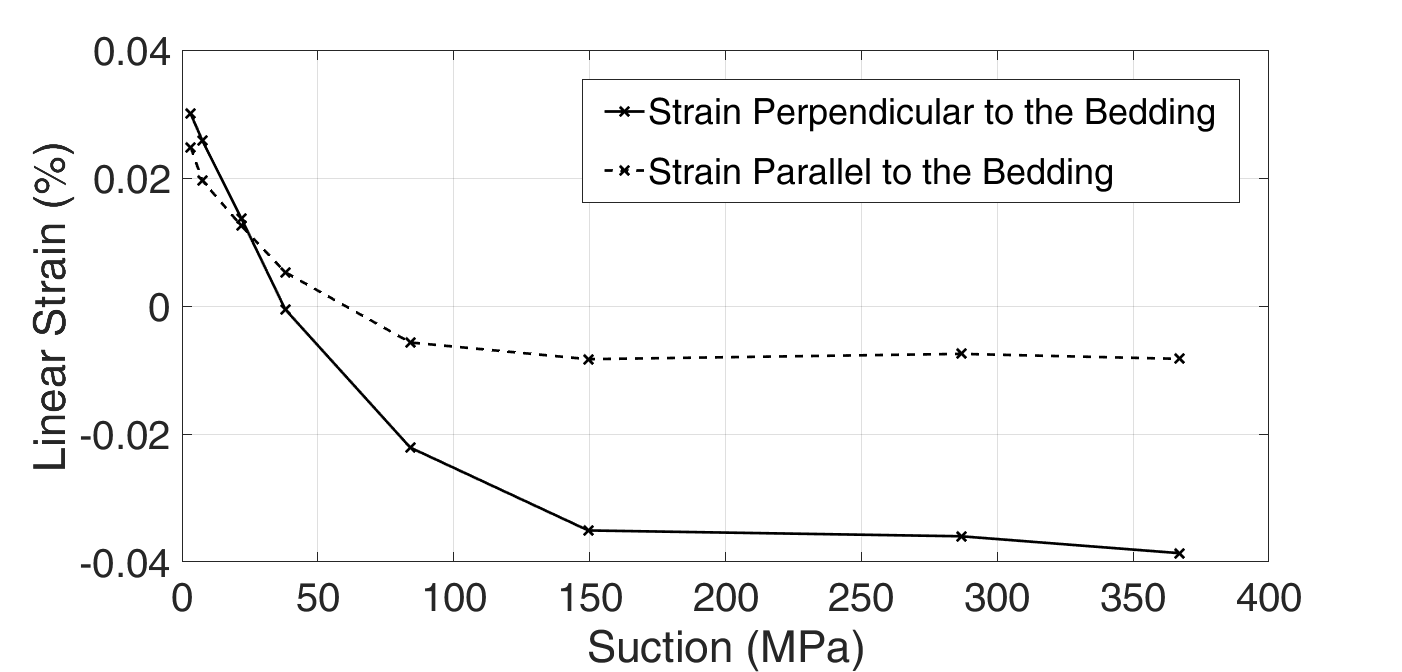
\includegraphics[width=5cm,height=4cm]{figures/Amir_ME6_Strain.png}
\subcaption{}
\label{fig:Amir_ME6_Strain}
\end{subfigure}
\hfill
\begin{subfigure}[c]{0.48\textwidth}
\centering
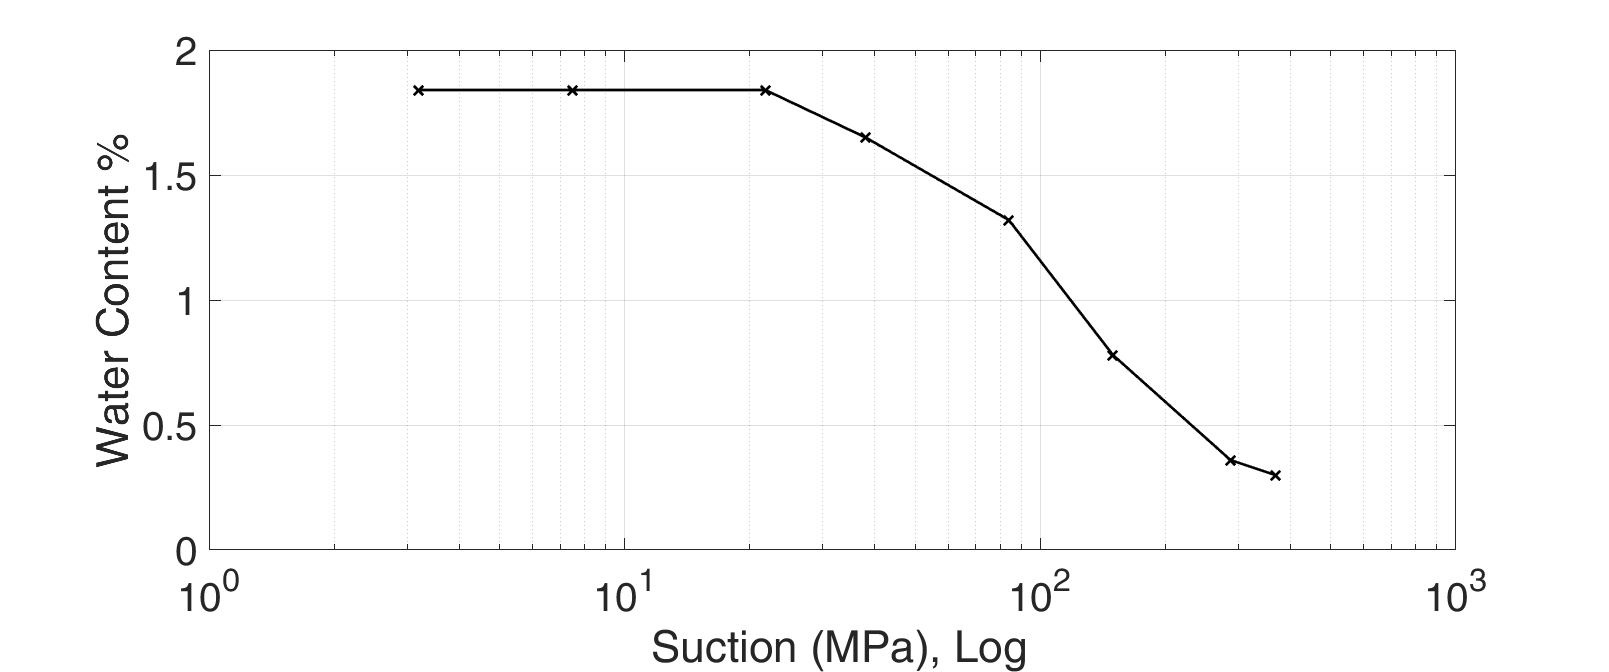
\includegraphics[width=5cm,height=4cm]{figures/Amir_ME6_Water.png}
\subcaption{}
\label{fig:Amir_ME6_Water}
\end{subfigure}
\caption{The drying and wetting paths for Opalinus claystone (a) the suction vs. linear strains, (b) the suction vs. the water content}
\end{figure}


%------------------------------------------------------------------------------
\subsection{Model approaches}

The simulation results from each of the model methods, discrete element method (DEM), lattice element method (LEM) and phase field method (PFM) are described and the accuracy of numerical results for modeling the shrinkage process with change of linear or volumetric strains as well as the change of anisotropic hydraulic conductivity are investigated. 

\subsubsection*{Discrete-Element-Model (DEM)}
\todo{[IfG] Contribution planned?}

\subsubsection*{Lattice element model}

With the application of the integrated interface element \cite{Sattarietal2019b} the drying and wetting processes in the Opalinus claystone are simulated. The linear strain of the elements are calculated based on the experimental data. The initial hydraulic conductivity values are approximated according to the technical Report, Mont Terri 2008-04 as,

\begin{align}
\label{eq:LEM_ME6_1}
\begin{split}
K_\parallel=2\times{10}{^{-13}}\\\\\\\\\\K_\bot=0.6\times{10}{^{-13}}
\end{split}
\end{align}

While considering the cubic law for flow transfer through the porous medium, the hydraulic aperture or length of the interface element is calculated as,

\begin{align}
\label{eq:LEM_ME6_2}
\begin{split}
e=\sqrt(K\times12\times\upsilon/g)\\\\\e_\parallel=4.95\times{10}{^{-10}}\\\\\\\ e_\bot=2.71\times{10}{^{-10}}
\end{split}
\end{align}

where $\upsilon=1.004\times{10}{^{-6}}$ and g=9.8. The domain is generated using the vectorizable lattice element with defined layers as described in previous sections (Figure \ref{fig:Amir_ME6_Lattice_Setup}). The interface length is defined based on \ref{eq:LEM_ME6_2}.

\begin{figure}[!ht]
\centering
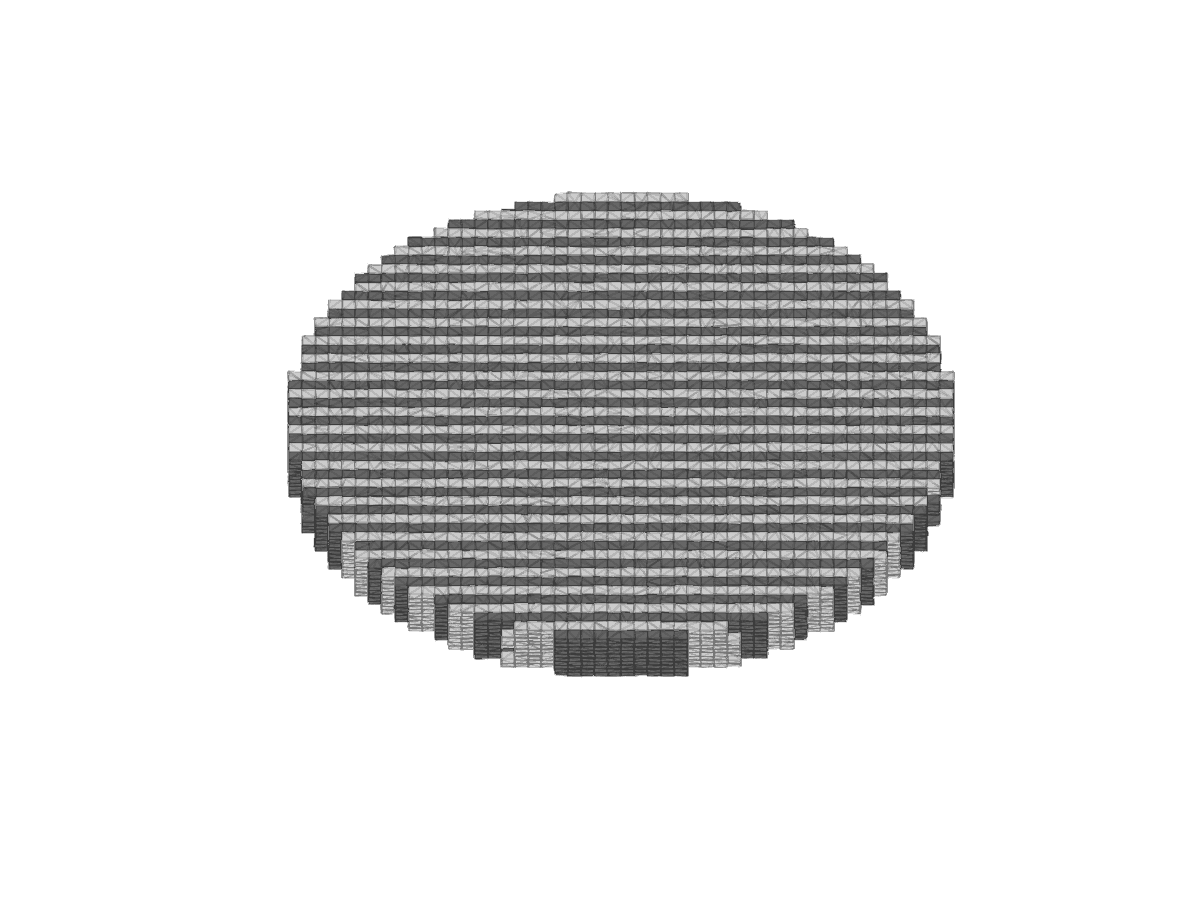
\includegraphics[width=0.75\textwidth]{figures/Amir_ME6_Lattice_Setup.png}
\caption{The generated domain for simulation of the drying and wetting processes}
\label{fig:Amir_ME6_Lattice_Setup}
\end{figure} 


%-----------------------------


\subsubsection*{Finite-Element-Method: Variational-Phase-Field (VPF)}
\todo{[UFZ] Contribution planned?}
FEM mesh~\ref{fig:ME5_VPF_setup}.

\begin{figure}[!ht]
\centering
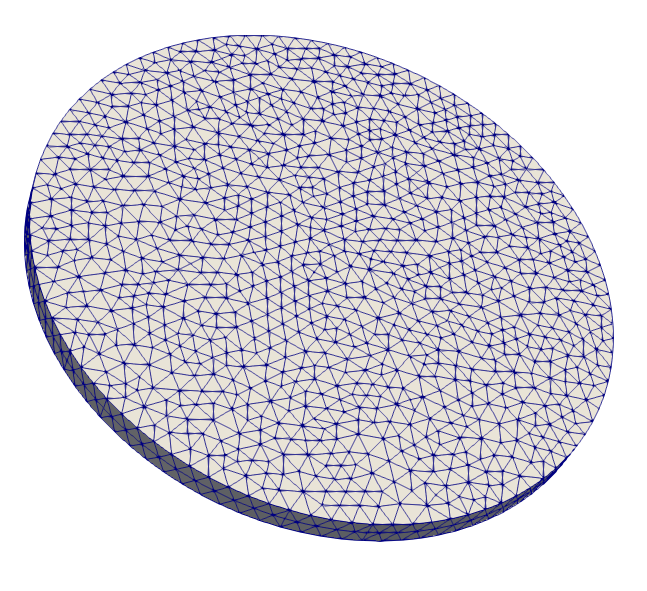
\includegraphics[width=0.75\textwidth]{figures/ME5_VPF_mesh.png}
\caption{The generated FEM mesh for shrinkage process}
\label{fig:ME5_VPF_setup}
\end{figure} 
%------------------------------------------------------------------------------
\subsection{Results and discussion}